\documentclass[a4paper]{article}


\usepackage[T1]{fontenc}    
\usepackage[utf8]{inputenc} 
\usepackage{textcomp}      
\date{} 					
\author{}                   
\usepackage{geometry}		
\geometry{ left=2cm, right=2cm, top=2cm, bottom=4cm, bindingoffset=5mm}

\usepackage{graphicx}
\usepackage{xcolor}
\usepackage{hyperref} 
\usepackage{fancyhdr}
\usepackage{amsmath}											
\pagestyle{fancy}
\fancyhf{}
\fancyhead[R]{2973140 - Felix Bühler  \\ 2893121 - Jan Leusmann \\  3141241 - Jamie Ullerich}
\fancyhead[L]{Scientific Visualisation \\ Sommersemester 2019 }
\renewcommand{\headrulewidth}{0.5pt} 				

\title{Exercise 5}

\begin{document}

\maketitle 
\thispagestyle{fancy}



\section*{Exercise 5.1 [3 Points] Delaunay Triangulation - Edge-Flip}

\begin{figure}[h!]
	\centering
	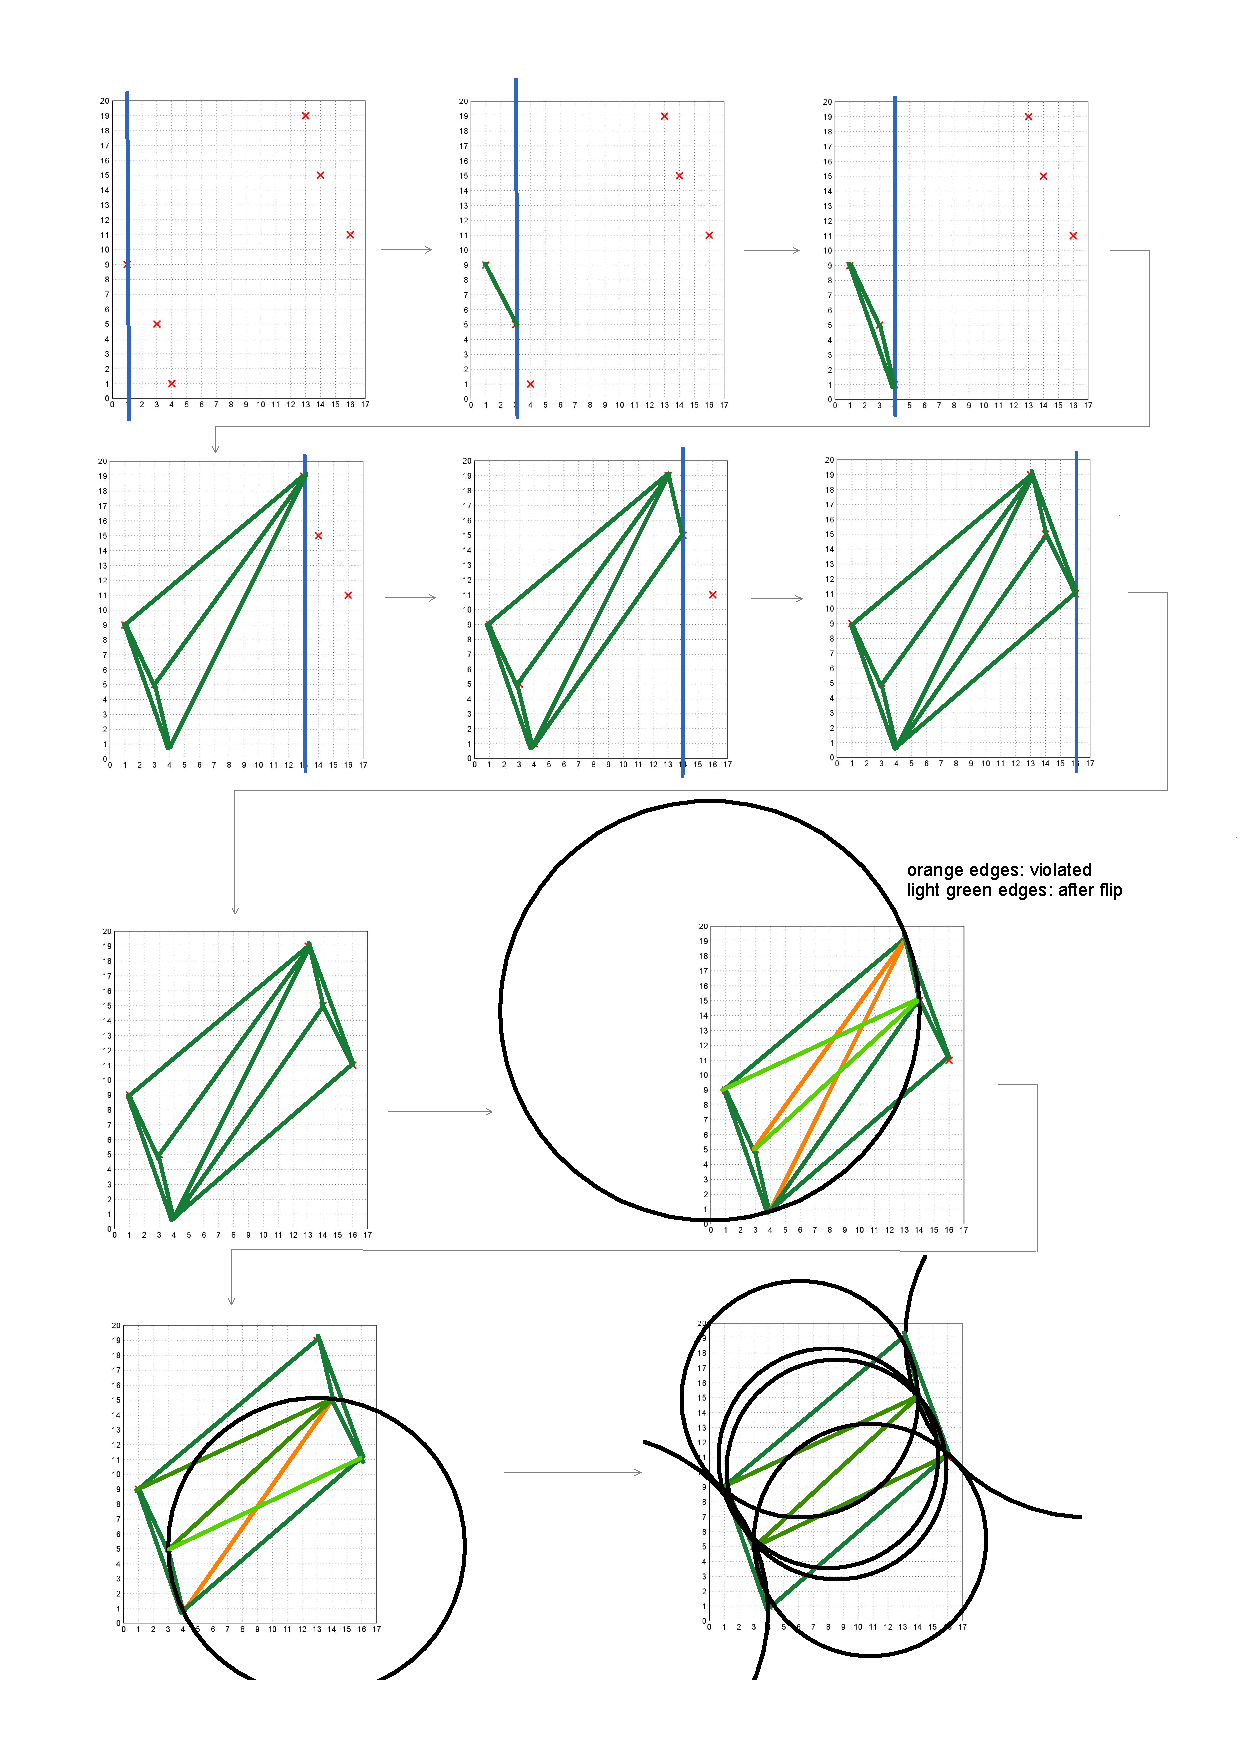
\includegraphics[width=0.79\linewidth]{delaunay.pdf}
	%\caption{}
	\label{fig:delaunay}
\end{figure}

\clearpage

\section*{Exercise 5.2 [3 Points] Inverse Distance Weighting}
$ P_7 $:\\
distances:
\begin{itemize}
	\item $ P_1 = \begin{Vmatrix}\begin{pmatrix}
	3 \\
	3
	\end{pmatrix}
	-
	\begin{pmatrix}
	2 \\
	2
	\end{pmatrix}\end{Vmatrix} = \sqrt{2} $
	\item $ P_2 = \begin{Vmatrix}
	\begin{pmatrix}
	3 \\
	3
	\end{pmatrix}
	-
	\begin{pmatrix}
	4 \\
	3
	\end{pmatrix}
	\end{Vmatrix} = \sqrt{5} $
	\item $ P_3 = \begin{Vmatrix}
	\begin{pmatrix}
	3 \\
	3
	\end{pmatrix}
	-
	\begin{pmatrix}
	4 \\
	5
	\end{pmatrix}
	\end{Vmatrix} = 1 $
	\item $ P_4 = \begin{Vmatrix}
	\begin{pmatrix}
	3 \\
	3
	\end{pmatrix}
	-
	\begin{pmatrix}
	5 \\
	5
	\end{pmatrix}
	\end{Vmatrix} = \sqrt{8} $
\end{itemize}
basis functions:
\begin{align*}
\phi_{1}
\begin{pmatrix}
3 \\
3
\end{pmatrix}
& =
\dfrac{
	\sqrt{2}^{-2}
}{
	\sqrt{2}^{-2}
	+
	\sqrt{5}^{-2}
	+
	1^{-2}
	+
	\sqrt{8}^{-2}
} \\
& = \dfrac{0.5}{0.5+1.+0.2+0.125} \\
& = \dfrac{0.5}{1.825}\\
& = 0.274
\end{align*}

\begin{align*}
\phi_{2}
\begin{pmatrix}
3 \\
3
\end{pmatrix}
& = \dfrac{0.2}{1.825}\\
& = 0.110
\end{align*}

\begin{align*}
\phi_{3}
\begin{pmatrix}
3 \\
3
\end{pmatrix}
& = \dfrac{1}{1.825}\\
& = 0.548
\end{align*}

\begin{align*}
\phi_{4}
\begin{pmatrix}
3 \\
3
\end{pmatrix}
& = \dfrac{0.125}{1.825}\\
& = 0.068
\end{align*}

\begin{align*}
f_{7}
\begin{pmatrix}
3 \\
3
\end{pmatrix}
& = 0.274 * 11 + 0.110 * 9 + 0.548 * 2 + 0.068 * 12\\
& = 5.916
\end{align*}

$ P_8 $:\\
distances:
\begin{itemize}
	\item $ P_2 $ = $ 2.5 $
	\item $ P_3 $ = $ 1.5 $
	\item $ P_4 $ = $ \sqrt{4.25} $
	\item $ P_5 $ = $ 1.5 $
	\item $ P_6 $ = $ \sqrt{4.25} $
\end{itemize}

basis functions:
\begin{align*}
\phi_{2}
\begin{pmatrix}
5.5 \\
3
\end{pmatrix}
& =
\dfrac{
	2.5^{-2}
}{
	2.5^{-2}
	+
	1.5^{-2}
	+
	\sqrt{4.25}^{-2}
	+
	1.5^{-2}
	+
	\sqrt{4.25}^{-2}
} \\
& = \dfrac{0.160}{0.160 + 0.444 + 0.235 + 0.444 + 0.235}\\
& = \dfrac{0.160}{1.52}\\
& = 0.105
\end{align*}

\begin{align*}
\phi_{3}
\begin{pmatrix}
5.5 \\
3
\end{pmatrix}
=
\phi_{5}
\begin{pmatrix}
5.5 \\
3
\end{pmatrix}
& = \dfrac{0.444}{1.52} = 0.293
\end{align*}

\begin{align*}
\phi_{4}
\begin{pmatrix}
5.5 \\
3
\end{pmatrix}
=
\phi_{6}
\begin{pmatrix}
5.5 \\
3
\end{pmatrix}
& = \dfrac{0.235}{1.52} = 0.155
\end{align*}

\begin{align*}
f_{8}
\begin{pmatrix}
5.5 \\
3
\end{pmatrix}
& = 0.105 * 9 + 0.293 * 2 + 0.155 * 12 + 0.293 * 8 + 0.155 * 13\\
& = 7.75
\end{align*}

\section*{Exercise 5.3 [1 Points] Interpolation inside a prism}
\begin{itemize}
	\item Get barycentric coordinates for upper an lower triangle we will get $ \alpha, \beta, \gamma $ for each triangle
	\item plug these into the formula and get the interpolated values for $ P_{upper} $ and $ P_{lower} $
	\item linear interpolation between $ P_{upper} $ and $ P_{lower} $ with inverse distance
\end{itemize}

\section*{Exercise 5.4 [5 Points] Paraview: Simple Gradient Plugin}
--
	
\end{document}